% Generated by bevy_zeroverse_publication timing-study; do not edit.
\section{Procedural pipeline and measured cost}
\label{sec:pipeline}
Figure~\ref{fig:pipeline-engine} follows the production path from seeded programs to completed views. Immutable architecture, furnishing and person assemblies are constructed once. The same triangles supply transport and rendering. A shared pool with at most four dedicated preparation threads executes independent builders; scoped callers can also execute queued work. Large BVH subtrees use a separate shared pool of up to four threads. Ordered results and reserved mesh handles preserve seed identity. Material preparation overlaps geometry transport, group planning and mesh/tangent realization. Only referenced material variants are prepared. Supported material maps and their mip chains are baked once on the GPU; remaining programs use the CPU oracle. Native room lookahead overlaps preparation, bounded speculative uploads and static lighting with current capture, without promoting future scene entities early. The browser uses cooperative yields in place of native worker parallelism; yields keep the event loop responsive but do not provide CPU parallelism.

\subsection{Protocol and accounting}
Measurements use an Intel Core i9-12900K (24 logical CPUs) and NVIDIA RTX PRO 6000 Blackwell Workstation Edition using Vulkan. Rust 1.100.0-nightly (2026-08-31 toolchain), native x86-64 Linux, optimized dev profile (opt-level 3; debug information disabled), multi\_threaded with default features disabled. Existing Gekko training and capture processes remained active; no other local qualification or compiler ran during the measured timing protocol. Device telemetry is board-wide and includes those other processes.. These are shared-machine measurements, not isolated hardware limits or a training-throughput benchmark. The receipt binds source SHA256 \texttt{8b9386343019c7a1}, package versions, exact configuration, input hashes and every measured seed. No geometry, texture resolution, shadow quality or GI-ray budget is reduced for this study. Static AnnyBody people are sampled at density 0.25; ARDY inference is disabled.

The CPU-only study samples 64 consecutive rooms, seeds 400--463, with 4 separate warm-up rooms. It invokes the same preparation entry point as capture, including camera sampling, layout validation, geometry, material recipes, transport, reflections and lighting requests. It prepares GPU requests without executing them and cannot measure rendered throughput. Table~\ref{tab:pipeline-stages} partitions one future's monotonic wall lifetime into disjoint intervals. Values include scheduling/waiting within a stage, not CPU core time. Relative shares divide summed stage durations by summed preparation lifetimes; percentiles use nearest rank. Concurrent branch times and different rooms must not be summed into this partition.

\begin{figure}[htbp]\centering
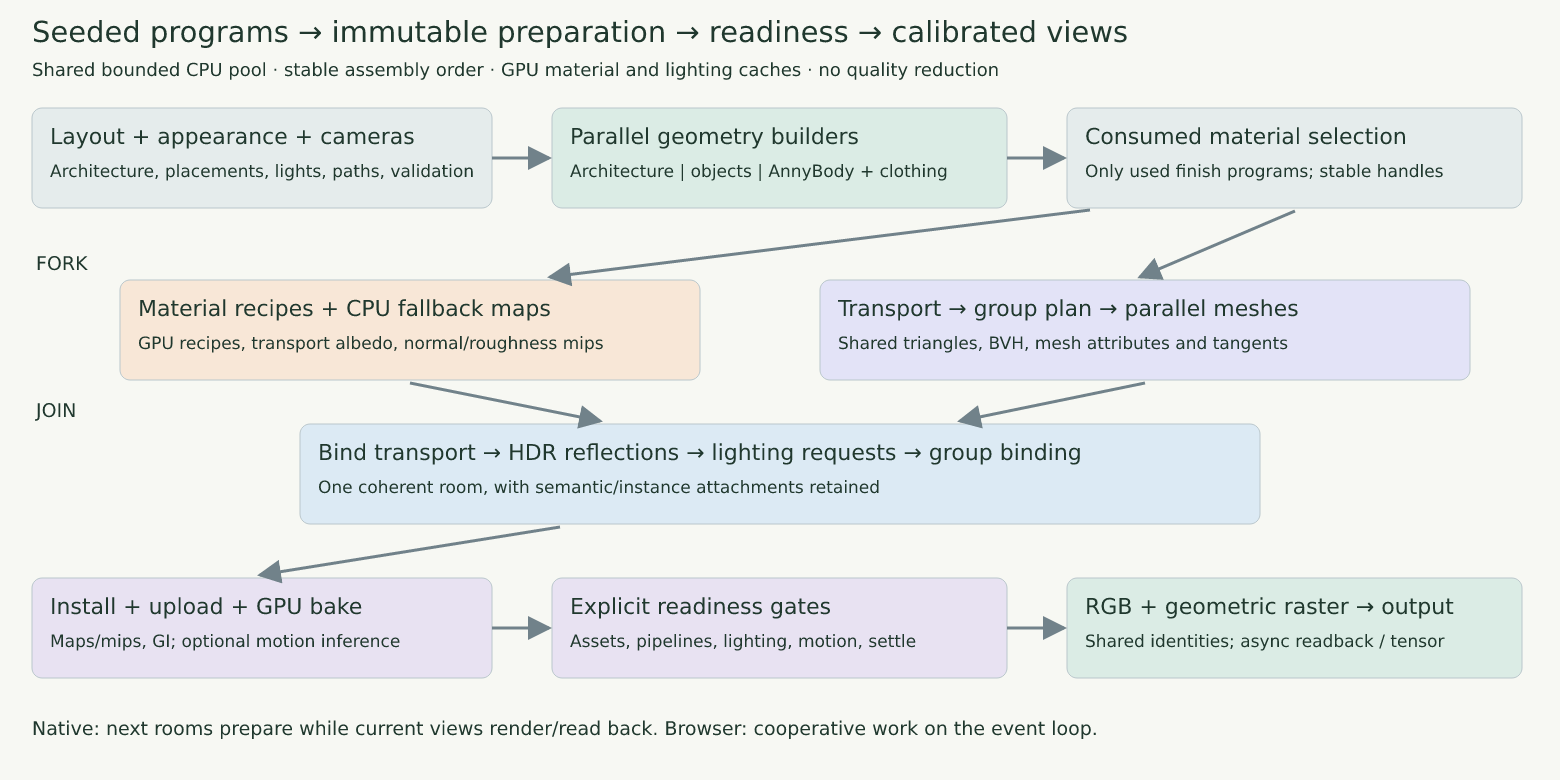
\includegraphics[width=\linewidth]{generated/pipeline_engine.png}
\caption{Production dependencies. The fork/join overlaps CPU material work with transport and mesh realization; GPU maps and lighting finish behind explicit readiness gates. Optional human inference is a separate gate. Consecutive-room lookahead spans these stages; the layout does not imply serial execution of whole rooms.}
\label{fig:pipeline-engine}\end{figure}

\begin{table}[htbp]\centering\small
\begin{tabular}{lrrrr}\toprule
Preparation phase & Mean (ms) & Median (ms) & p95 (ms) & Share (\%)\\\midrule
Layout and appearance & 2.28 & 1.70 & 6.03 & 0.26 \\
Camera paths and overlap & 88.56 & 43.53 & 303.98 & 10.04 \\
Layout validation & 10.09 & 8.71 & 21.05 & 1.14 \\
Motion planning & 0.00 & 0.00 & 0.00 & 0.00 \\
Geometry assemblies & 46.06 & 43.66 & 77.68 & 5.22 \\
Consumed material selection & 0.14 & 0.12 & 0.23 & 0.02 \\
Materials / transport / meshes & 543.58 & 499.47 & 871.16 & 61.60 \\
Transport material binding & 7.14 & 6.99 & 11.29 & 0.81 \\
HDR reflection environment & 148.67 & 131.76 & 266.23 & 16.85 \\
Lighting bake preparation & 32.07 & 30.00 & 62.58 & 3.63 \\
Serial mesh tail (Wasm) & 0.00 & 0.00 & 0.00 & 0.00 \\
Render group binding & 0.18 & 0.16 & 0.27 & 0.02 \\
Scheduling and bookkeeping & 3.66 & 3.67 & 6.93 & 0.41 \\
\midrule Total & 882.44 & 804.79 & 1485.02 & 100.00 \\
\bottomrule\end{tabular}
\caption{CPU preparation with production GPU material recipes, three square-aspect cameras and native Auto quality. The material/transport/mesh row counts the union once. Asset installation, actual GPU bakes, rendering and readback are downstream.}\label{tab:pipeline-stages}\end{table}

\subsection{Completed capture and bounded concurrency}
Each native capture run regenerates rooms and delivers three 512$\times$512 views at one timestep in RGB, depth, position, normal, semantic and co-visibility modes. Full native shadows, SSAO, GPU materials and 256-ray/probe GI remain enabled. The default three-room lookahead is used. The streaming denominator includes validation, diagnostic JSONL writes and asset/sample destruction: preparation can advance during these operations. No image compression, dataset encoding or Burn tensor handoff is measured. Capture latency covers request to complete sample; it differs from streaming wall cost. GPU timestamp instrumentation is disabled in throughput runs.

\begin{table}[htbp]\centering\small
\begin{tabular}{lrrrr}\toprule
Workload & Rooms & Wall rooms/s & Median (ms) & p95 (ms)\\\midrule
CPU preparation, 1 in flight & 64 & 1.129 & 804.8 & 1485.0 \\
CPU preparation, 4 in flight & 64 & 2.324 & 1570.9 & 2519.6 \\
Completed capture, run 1 & 64 & 0.995 & 964.2 & 1734.3 \\
Completed capture, run 2 & 64 & 1.081 & 839.9 & 1980.7 \\
\bottomrule\end{tabular}
\caption{Different denominators: CPU-only preparation emits immutable asset plans; completed capture emits all requested planes. Repeated capture runs expose shared-machine variability. Neither rate includes downstream training.}\label{tab:pipeline-throughput}\end{table}
Capture run 1 excludes 16 warm-up rooms; setup took 1.71 s and the first room took 5.71 s. The measured stream delivered 2.99 views/s; capture spans occupied 99.27\% of stream wall time. These spans overlap future-room work. Main-world installation records deferred ECS commands and asset insertion, not their later execution or upload.

Capture run 2 excludes 16 warm-up rooms; setup took 2.02 s and the first room took 5.16 s. The measured stream delivered 3.24 views/s; capture spans occupied 99.15\% of stream wall time. These spans overlap future-room work. Main-world installation records deferred ECS commands and asset insertion, not their later execution or upload.

\subsection{Hot spots and next optimization targets}
The largest measured preparation windows are Materials / transport / meshes, HDR reflection environment and Camera paths and overlap (Figure~\ref{fig:pipeline-profile}). They are observations of this workload, not universal cost ratios.
Within the parallel asset window, mean material preparation is 306.9 ms, geometry transport construction is 349.2 ms, and mesh/tangent realization is 181.8 ms. Transport precedes meshes; that branch overlaps material work. Geometry builder service times are separately retained by architecture, object and person categories; their sums are not a CPU-utilization measurement.

Priority candidates are reducing triangle-staging and BVH-construction memory traffic, improving scheduling of the existing parallel transport subtrees, and GPU or batched reflection-environment synthesis. Camera visibility searches need independent rejection/attempt profiling before changing their budget: reducing the search budget can bias the camera distribution. Geometry assembly is separately measured, so finer-grained person/architecture scheduling should be pursued only when it is on the critical path. Any move of map or reflection work to the GPU must retain deterministic inputs, normal/roughness mip correctness, annotation alignment and measured completed capture throughput while training competes for the device. Pool expansion can increase contention; more workers are not automatically faster. Broad caching keyed only by material category would reduce procedural diversity and is not an acceptable optimization.

Render-preparation, GI/material readiness, settling and readback event-loop buckets are retained in the receipt. A bucket names the blocker observed before an update; it is not an exclusive CPU or GPU execution timer. Asynchronous GPU diagnostics can arrive late and contain nested intervals, so they are not summed into per-room GPU time. A GPU timeline profiler is still needed to attribute submission gaps, uploads and individual kernels. This study does not measure isolated GPU utilization, device-to-device tensor throughput, motion inference or browser latency. Wasm compilation checks preserve the path; browser timing requires a separate hardware-WebGPU run.

\begin{figure}[htbp]\centering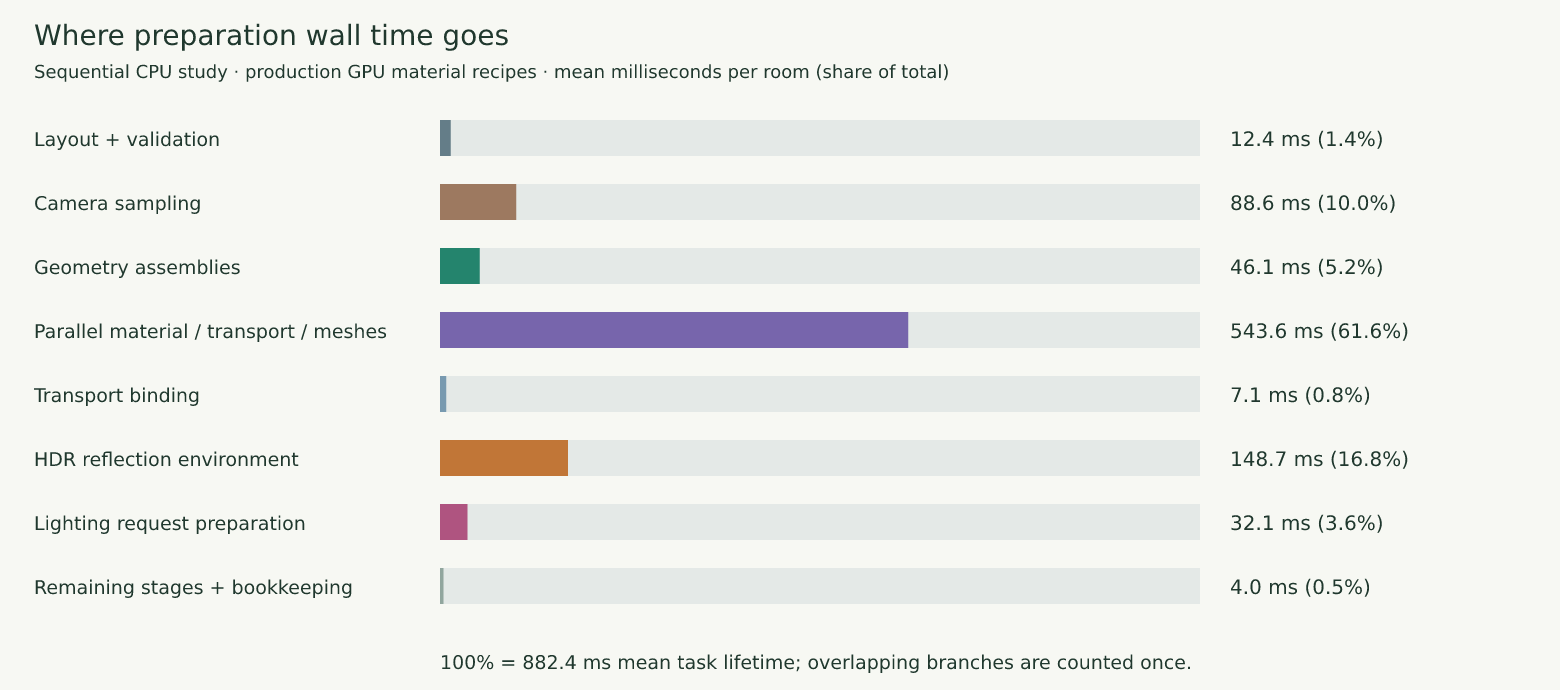
\includegraphics[width=\linewidth]{generated/pipeline_profile.png}
\caption{Mean per-room CPU preparation wall time and its relative partition for the sequential CPU study. Colors separate the major phases; the parallel window includes scheduling and both branches, exactly once. This is not a utilization chart.}\label{fig:pipeline-profile}\end{figure}
\clearpage
